% Template for Latex
% Document author - Nagendra Krishnamurthy

\documentclass[12pt]{article}

\setlength{\textwidth}{6.5in}
\setlength{\textheight}{8.75in}
\setlength{\evensidemargin}{0in}
\setlength{\oddsidemargin}{0in}
\setlength{\topmargin}{0in}

\setlength{\parindent}{0pt}
\setlength{\parskip}{0.1in}

\title{NSEG-5984 Monte Carlo Methods for Particle Transport}
%\subtitle{Homework 1}
\author{Nagendra Krishnamurthy}

% Uncomment for double-spaced document.
% \renewcommand{\baselinestretch}{2}

\usepackage[latin1]{inputenc}
\usepackage{tikz}
\usetikzlibrary{shapes,arrows}
\usepackage{epstopdf}
% \usepackage{epsf}
% \usepackage{glossaries}
\usepackage{graphicx}
\usepackage{scalefnt}
\usepackage{amsmath}

\definecolor{Brown}{cmyk}{0,0.81,1,0.60}
\definecolor{OliveGreen}{cmyk}{0.64,0,0.95,0.40}
\definecolor{CadetBlue}{cmyk}{0.62,0.57,0.23,0}
\definecolor{lightlightgray}{gray}{0.9}

\usepackage{listings}
\lstset{frame=shadowbox, rulesepcolor=\color{blue}}
\lstset{ %
language=[90]Fortran,           % the language of the code
basicstyle=\scriptsize\ttfamily,           % the size of the fonts that are used for the code
%numbers=left,                  % where to put the line-numbers
numberstyle=\scriptsize,      % the size of the fonts that are used for the line-numbers
stepnumber=2,                   % the step between two line-numbers. If it's 1, each line 
                                % will be numbered
numbersep=5pt,                  % how far the line-numbers are from the code
backgroundcolor=\color{lightlightgray},  % choose the background color. You must add \usepackage{color}
showspaces=false,               % show spaces adding particular underscores
showstringspaces=false,         % underline spaces within strings
showtabs=false,                 % show tabs within strings adding particular underscores
frame=single,                   % adds a frame around the code
tabsize=2,                      % sets default tabsize to 2 spaces
captionpos=b,                   % sets the caption-position to bottom
breaklines=true,                % sets automatic line breaking
breakatwhitespace=false,        % sets if automatic breaks should only happen at whitespace
title=\lstname,                 % show the filename of files included with \lstinputlisting;
                                % also try caption instead of title
escapeinside={\%*}{*)},         % if you want to add a comment within your code
keywordstyle=\color{OliveGreen}, % Keywords font ('*' = uppercase)
morekeywords={*,...}           % if you want to add more keywords to the set
}
% \usepackage{natbib}

% \makeglossaries

% \newglossaryentry{cd}{name=$C_D$,description={Coefficient of drag}}
% \newglossaryentry{cl}{name=$C_L$,description={Coefficient of lift}}

\begin{document}

Source codes for both the problems are provided at the end of the
assignment.

\textbf{Problem 1:}

The following tables provide results obtained from the analog code.
The two cases - 10 and 50 regions used for the calculations are
provided. For the second case, only the figure is provided. The
following conclusions can be made from the results:
\begin{itemize}
  \item It is seen that as the number of regions are increased, the
    estimation of the scalar flux establishes a more or less constant
    value throughout the region.
  \item The above behavior is in-line with the variation of relative
    error. The relative error when 10 regions are considered increases
    as the region moves away from the particle source, when 50 regions
    are considered, the relative error is more or less constant.
  \item Both the types of estimators provide similar estimates of
    scalar flux in most of the regions.
\end{itemize}

\begin{center}
  \begin{tabular}{|c|c|c|c|c|}
    \hline
    & \multicolumn{2}{c|}{\textbf{Collision estimator}}
    & \multicolumn{2}{c|}{\textbf{Path length estimator}}\\
     \cline{2-5}
    \hline
    Region number & Scalar flux & Relative error & Scalar flux &
    Relative error\\
    \hline
    1	 & 1.50E+00 & 2.15E-03 & 1.38E+00 & 2.06E-03 \\
    2	 & 1.00E+00 & 4.51E-03 & 7.78E-01 & 1.77E-03 \\
    3	 & 5.19E-01 & 3.81E-03 & 4.14E-01 & 7.18E-03 \\
    4	 & 2.63E-01 & 4.15E-03 & 2.42E-01 & 3.71E-03 \\
    5	 & 1.45E-01 & 1.08E-02 & 1.03E-01 & 8.53E-03 \\
    6	 & 8.70E-02 & 8.29E-03 & 5.79E-02 & 7.47E-03 \\
    7	 & 4.50E-02 & 1.20E-02 & 2.57E-02 & 9.84E-03 \\
    8	 & 3.00E-02 & 1.33E-02 & 1.44E-02 & 1.33E-02 \\
    9	 & 1.20E-02 & 1.62E-02 & 7.55E-03 & 2.00E-02 \\
    10 & 1.50E-02 & 1.60E-02 & 5.65E-03 & 2.11E-02 \\
    \hline
  \end{tabular}
  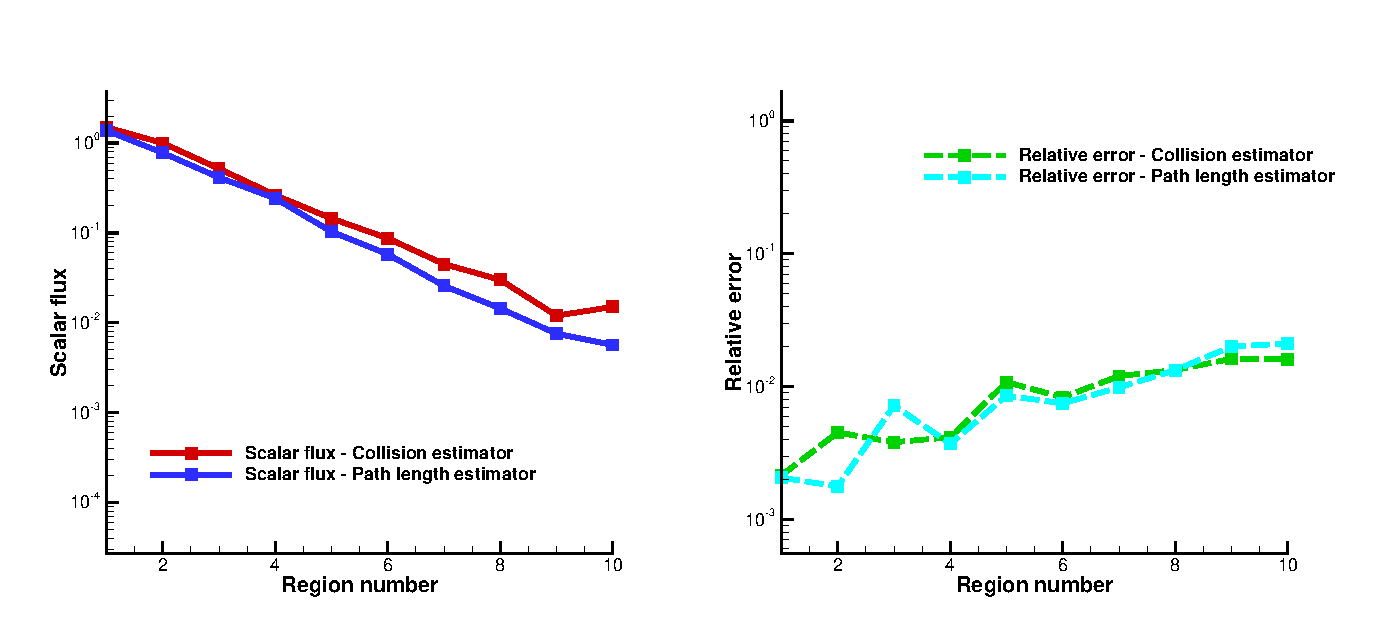
\includegraphics[width=1.0\textwidth]{problem1_10.eps}
\end{center}

\begin{center}
  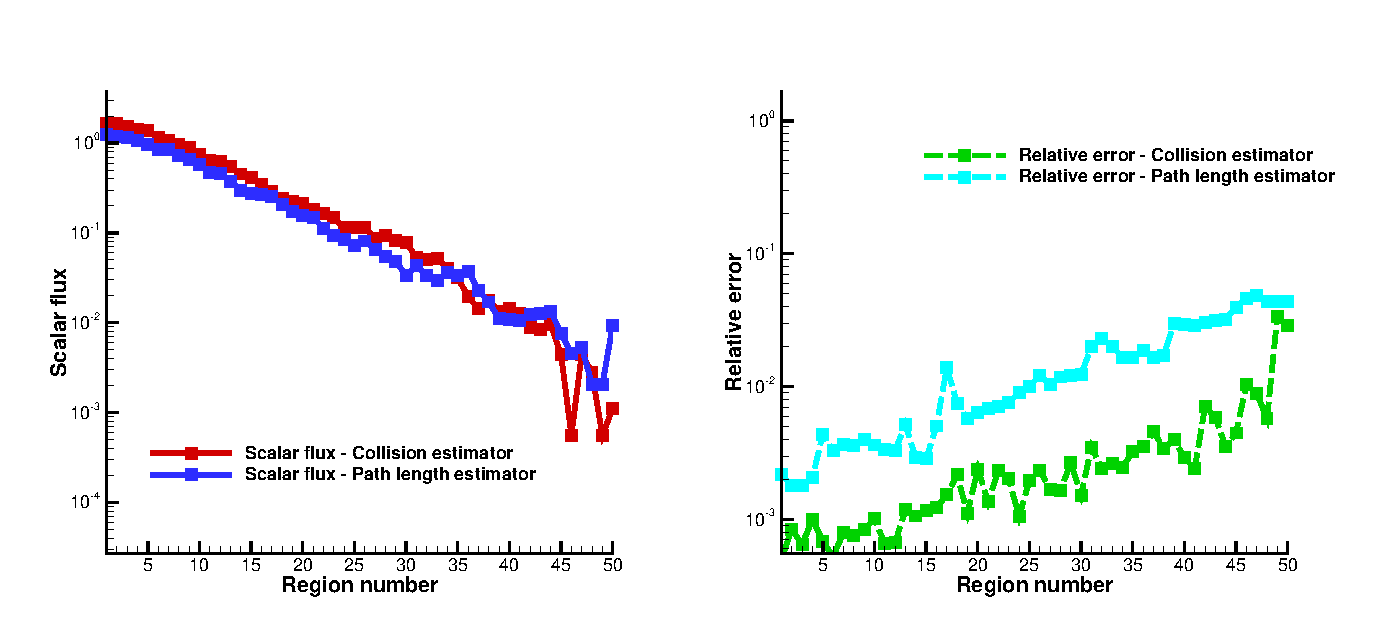
\includegraphics[width=1.0\textwidth]{problem1_50.eps}
\end{center}

Source code:
\lstinputlisting{problem_1.f90}

\textbf{Problem 2:}

\begin{center}
  \begin{tabular}{|c|c|c|c|c|}
    \hline
    & \multicolumn{2}{c|}{\textbf{Collision estimator}}
    & \multicolumn{2}{c|}{\textbf{Path length estimator}}\\
     \cline{2-5}
    \hline
    Region number & Scalar flux & Relative error & Scalar flux &
    Relative error\\
    \hline
    1	 & 7.28E-01 & 2.67E-03 & 6.23E-01 & 1.21E-03 \\
    2	 & 2.99E-01 & 3.51E-03 & 1.94E-01 & 2.86E-03 \\
    3	 & 1.04E-01 & 3.97E-03 & 1.27E-01 & 4.60E-03 \\
    4	 & 3.33E-02 & 6.42E-03 & 2.34E-02 & 5.39E-03 \\
    5	 & 1.41E-02 & 9.24E-03 & 1.90E-02 & 5.59E-03 \\
    6	 & 6.07E-03 & 1.36E-02 & 4.22E-03 & 7.59E-03 \\
    7	 & 1.59E-03 & 1.85E-02 & 2.88E-03 & 7.77E-03 \\
    8	 & 5.74E-04 & 1.32E-02 & 4.58E-04 & 1.55E-02 \\
    9	 & 3.39E-04 & 2.80E-02 & 3.82E-04 & 1.57E-02 \\
    10 & 1.92E-04 & 2.84E-02 & 7.52E-05 & 1.89E-02 \\
    \hline
  \end{tabular}
  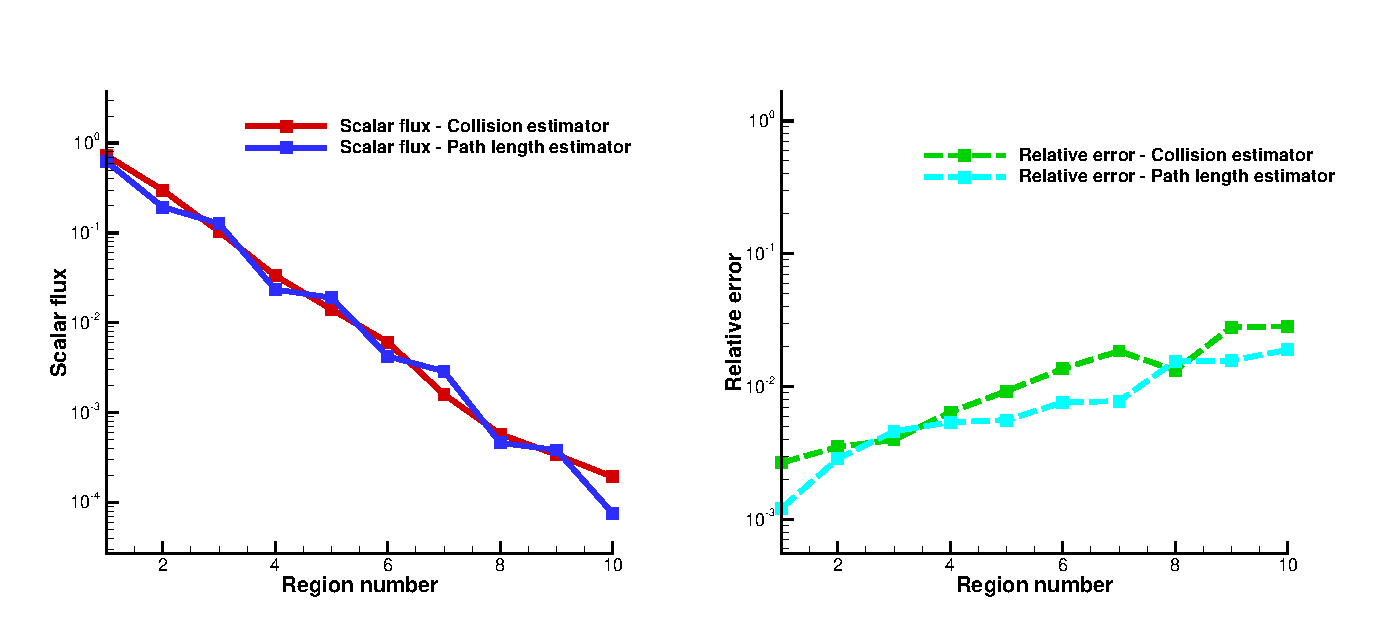
\includegraphics[width=1.0\textwidth]{problem2_10.eps}
\end{center}

\begin{center}
  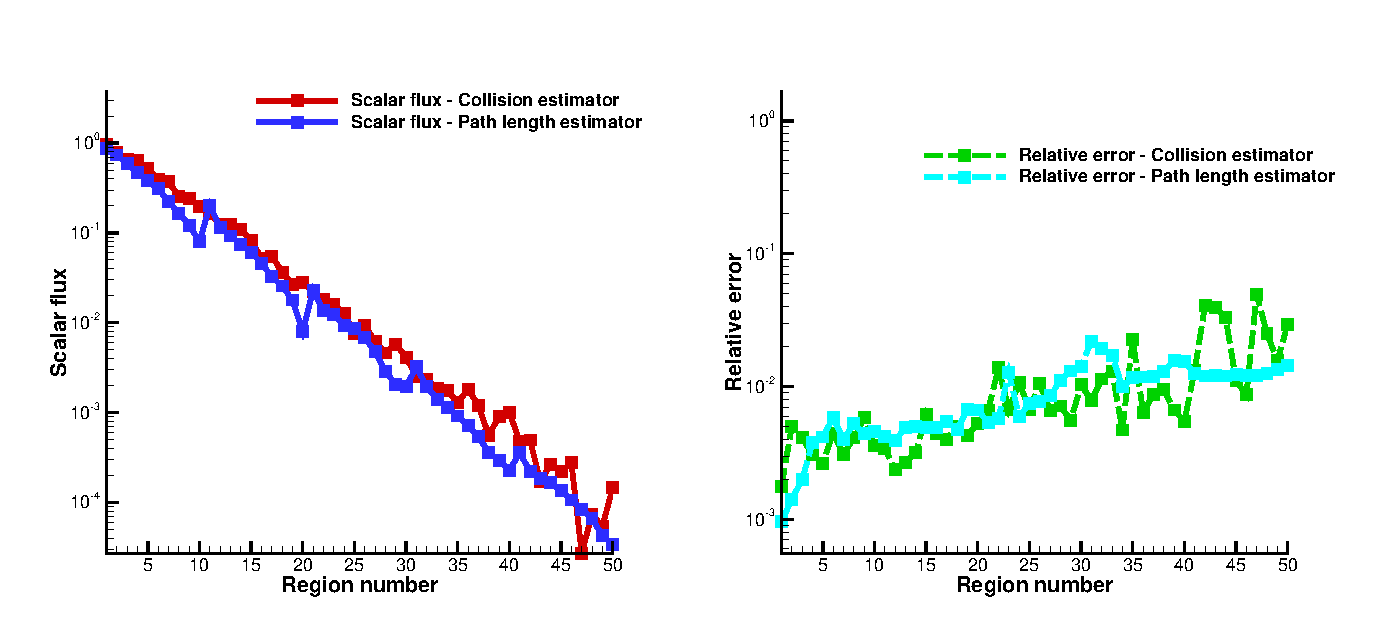
\includegraphics[width=1.0\textwidth]{problem2_50.eps}
\end{center}

Source code:
\lstinputlisting{problem_2.f90}


% \bibliographystyle{plainnat}
% \bibliography{path_to_bibliography}
% \printglossaries

\end{document}
